\section{Essential$<$ Data, Sets\-Type $>$ Class Template Reference}
\label{class_essential}\index{Essential@{Essential}}
Functor representing the predicate being frequent essential.  


{\tt \#include $<$Essential.hxx$>$}

Inheritance diagram for Essential$<$ Data, Sets\-Type $>$::\begin{figure}[H]
\begin{center}
\leavevmode
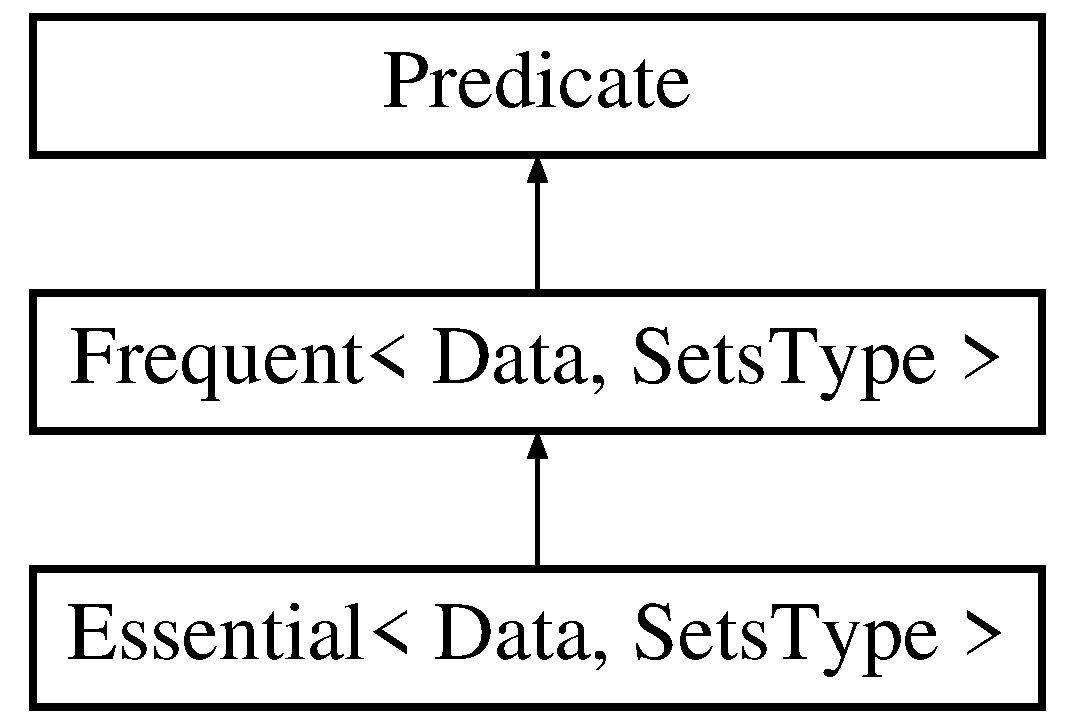
\includegraphics[height=3cm]{class_essential}
\end{center}
\end{figure}
\subsection*{Public Member Functions}
\begin{CompactItemize}
\item 
{\bf Essential} (Data \&indb, int in\-Minsup)
\begin{CompactList}\small\item\em Constructor. \item\end{CompactList}\item 
{\bf $\sim$Essential} ()\label{class_essential_a4f54ab8615df753dffc0a4d64af6c63}

\begin{CompactList}\small\item\em Destructor. \item\end{CompactList}\item 
template$<$class Iterator, class Measure$>$ bool {\bf operator()} (Iterator itemset\-It, Measure \&mes\-Cand)
\begin{CompactList}\small\item\em Operator that test if an itemet is frequent or not. \item\end{CompactList}\end{CompactItemize}


\subsection{Detailed Description}
\subsubsection*{template$<$class Data, class Sets\-Type$>$ class Essential$<$ Data, Sets\-Type $>$}

Functor representing the predicate being frequent essential. 

This functor test if an itemset is frequent and essential. This functor process the support and the disjunction before pruning. We suppose that the data has the same internal encoding than the candidates (ie, the first item met is recoded in \char`\"{}0\char`\"{}, the second in \char`\"{}1\char`\"{}, ...).

The methods of this predicate are specific to tries data structure ({\bf PTree}{\rm (p.\,\pageref{class_p_tree})} for the candiates and {\bf Tatree}{\rm (p.\,\pageref{class_tatree})} for the transactions). For the moment, this functor can only be used when using a levelwise exploration of the search space ({\bf Apriori}{\rm (p.\,\pageref{class_apriori})}) since it checks for subsets already generated.

The template parameter Data is the type of the transactional database. The template parameter Sets\-Type is the type of the items. 



\subsection{Constructor \& Destructor Documentation}
\index{Essential@{Essential}!Essential@{Essential}}
\index{Essential@{Essential}!Essential@{Essential}}
\subsubsection{\setlength{\rightskip}{0pt plus 5cm}template$<$class Data, class Sets\-Type$>$ {\bf Essential}$<$ Data, Sets\-Type $>$::{\bf Essential} (Data \& {\em indb}, int {\em in\-Minsup})\hspace{0.3cm}{\tt  [inline]}}\label{class_essential_c47b2c4a5a736b4f0d6d6da070d3f3ed}


Constructor. 

\begin{Desc}
\item[Parameters:]
\begin{description}
\item[{\em indb}]the transactional database \item[{\em in\-Minsup}]the absolute minimum support threshold \end{description}
\end{Desc}


\subsection{Member Function Documentation}
\index{Essential@{Essential}!operator()@{operator()}}
\index{operator()@{operator()}!Essential@{Essential}}
\subsubsection{\setlength{\rightskip}{0pt plus 5cm}template$<$class Data, class Sets\-Type$>$ template$<$class Iterator, class Measure$>$ bool {\bf Essential}$<$ Data, Sets\-Type $>$::operator() (Iterator {\em itemset\-It}, Measure \& {\em mes\-Cand})\hspace{0.3cm}{\tt  [inline]}}\label{class_essential_e6a89fa2543fe441619066b0f4f6323b}


Operator that test if an itemet is frequent or not. 

\begin{Desc}
\item[Parameters:]
\begin{description}
\item[{\em itemset\-It}]iterator (or pointer) on the itemset to test wrt the predicate \item[{\em mes\-Cand}]value of the support of the itemset \end{description}
\end{Desc}


Reimplemented from {\bf Frequent$<$ Data, Sets\-Type $>$} {\rm (p.\,\pageref{class_frequent_82e02ab1cf1749ea52e9603dc06a5d15})}.

The documentation for this class was generated from the following file:\begin{CompactItemize}
\item 
F:/i\-Zi/problems/essential/Essential.hxx\end{CompactItemize}
